\documentclass[]{article}
\usepackage{graphicx}
\usepackage{amsmath}
\graphicspath{ {../figures/} }

\begin{document}

\title{Title}
\author{Author}
\date{Today}
\maketitle

\section{Problem definition } 

In this project, we aim to produce a model which outputs a sequence of sketch and extrude steps that transforms that recreates a shape with target geometry $G_{T}$. \\

The image below shows an example: 

\begin{figure}
	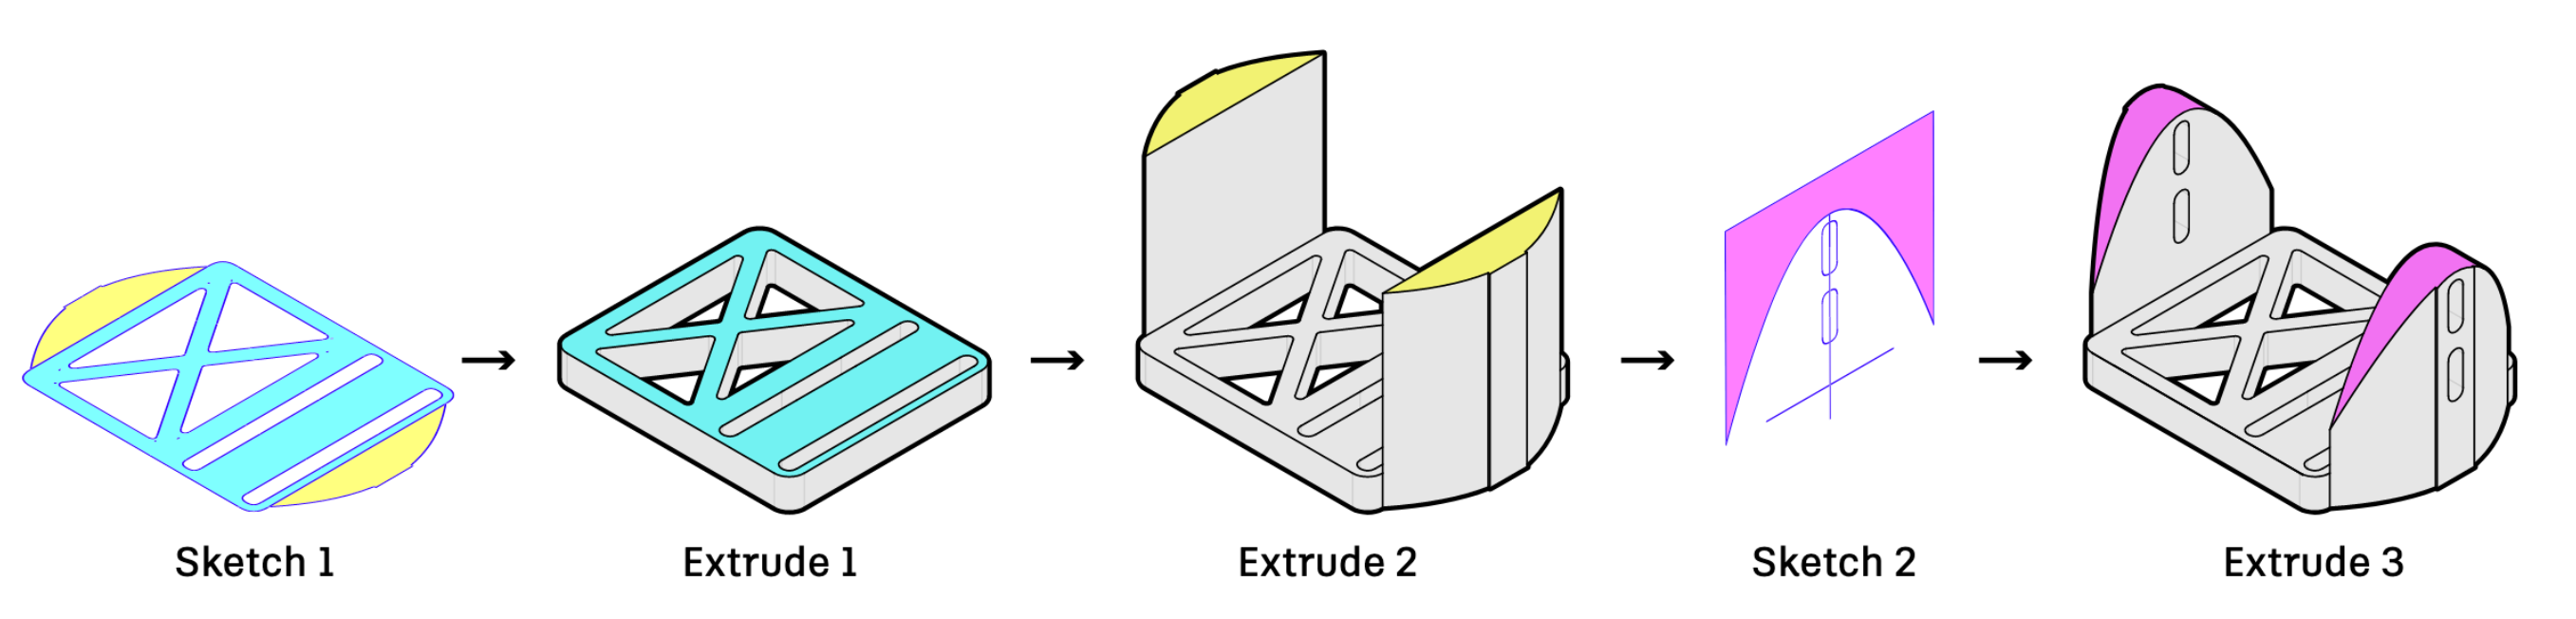
\includegraphics[width=\textwidth]{sketch-extrude} 
	\caption{Sample sketch and extrude sequence}
\end{figure}

The first step (left) is sketching the outline of the part, followed by an extrude step to give it volume. Then, another extrude step raises the edges and finally, an intersection is performed to obtain the final part. The goal of the model is to reconstruct the steps given the final representation. 

The authors of the dataset note that the steps taken to obtain the final representation is not necessarily unique, and therefore suggest the use of a conciseness metric to penalize overly complex sketch and extrude sequences alongside the “Intersection over Union” and “exact reconstruction loss which capture how accurate the reconstruction of the part is.

\section{Description}

The data consists of 8625 parts created using two operations: sketch and extrude. For each part, the dataset contains a metadata file describing the geometry of the sketches and the parameters of the extrusions. That is, for each part there is a sequence of steps that were taken to go from the original sketch to the finished part.

The metadata files describing the geometry and sketch/extrusion sequence are given in JSON format, as well as additional files in application specific formats.

\section{Related work}

In the paper accompanying the dataset, the authors present a novel learning architecture for recovering the sketch and extrude sequence. First, they build a supervised dataset by combining a pair of geometries $	(G_{c} , G_{t})$ and a modelling action (sketch or extrude) from the data and perform maximum likelihood over the correct actions:

\begin{align}
E_{(G_c, G_t) \sim \mathcal{D}}  \left[ log \pi_\theta \left( \hat{a_c} | \left(G_{c},G_{t}\right)  \right) \right]
\end{align}

Second, rather than operating on images, the authors propose the use of two message-passing networks (henceforth, MPN) to encode the source and target geometries, respectively. Finally, dense layers are connected to the concatenated vectors from the MPNs to predict a target action. This architecture is depicted in \ref{fig:arch}.


\begin{figure}
	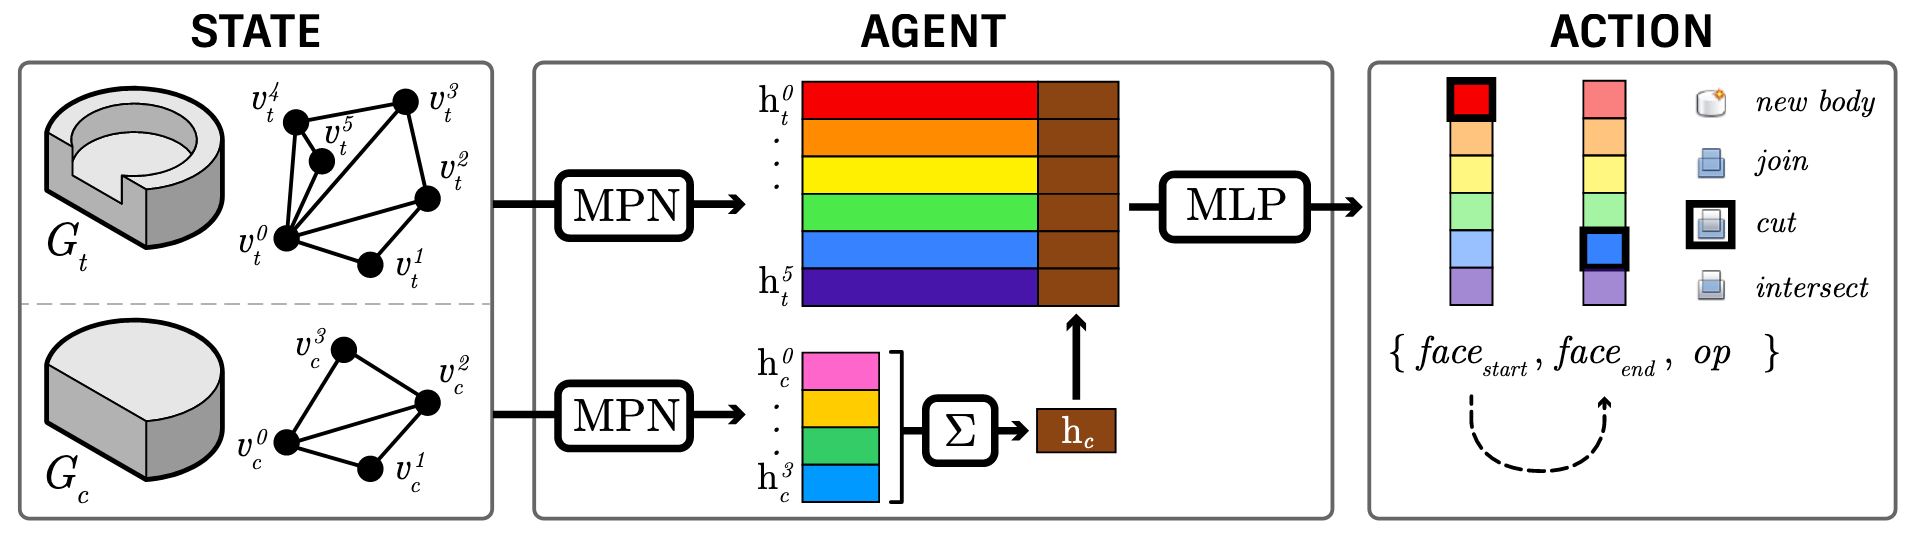
\includegraphics[width=\textwidth]{architecture} 
	\caption{Authors' network architecture}
	\label{fig:arch}
\end{figure}

\end{document}